\documentclass[9pt]{beamer}
\usepackage{tikz}
\usepackage{media9}
\usepackage{tabularx}
\usepackage{graphicx}
\usepackage{amsmath}

\usetikzlibrary{calc}
\graphicspath{ {./photos} }

\author{Hakim Rachidi}
\title{GYPT Basics}




\begin{document}
\begin{frame}
\titlepage
\end{frame}

\section{Allgemeines}

\begin{frame}
\frametitle{German Young Physicists' Tournament (GYPT)}


\begin{center}
{\large Fordert \color{orange} selbststaendiges \color{blue}wissenschaftliches \color{black} Arbeiten an physikalischen Phaenomenen, sowohl \underline{theoretisch} als auch \underline{experimentell}, von Schuelern}
\end{center}
\pause
\vfill

Ihr werdet ...
\begin{itemize}
\item eines der 17 Probleme aussuchen
\item Experimente planen und durchfuehren
\item Literatur (oder eigene Theorie) mit Experimenten vergleichen
\item Experiment und Theorie in Form einer 12-minutigen Praesentation als \emph{Reporter} praesentieren
\item mit dem \emph{Opponent} ueber die Ergebnisse diskutieren
\item als \emph{Opponent} die Ergebnisse eines gegnerischen Teams diskutieren
\end{itemize}
\end{frame}


\begin{frame}{Ziel dieser Praesentation}
\hspace*{-0.5cm}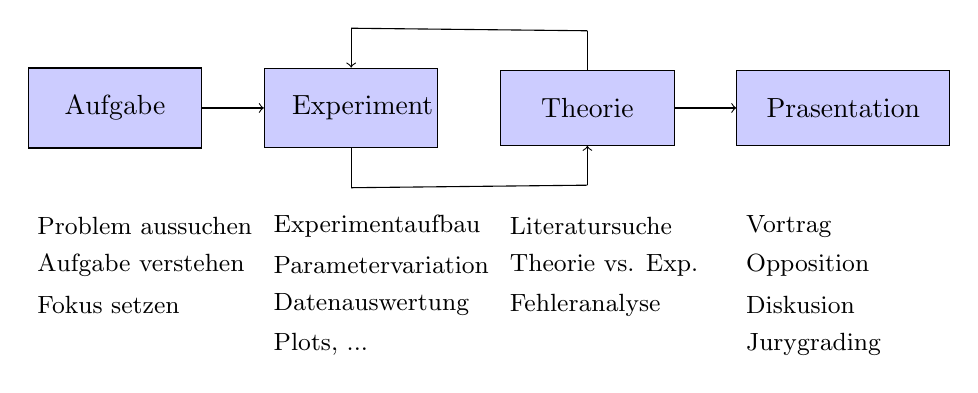
\begin{tikzpicture}

\node[draw, inner sep=10pt, text width=1.5cm, align=center, right, fill=blue!20!white] (2) at (-4, -2) {Aufgabe};
\node[draw, inner sep=10pt, text width=1.5cm, align=center, right, fill=blue!20!white] (3) at (-1, -2) {Experiment};
\node[draw, inner sep=10pt, text width=1.5cm, align=center, right, fill=blue!20!white] (4) at (2, -2) {Theorie};
\node[draw, inner sep=10pt, text width=2cm, align=center, right, fill=blue!20!white] (5) at (5, -2) {Prasentation};

\draw[->] (2.east) -- (3.west);
\draw[->] (4.east) -- (5.west);

\draw (4.north) -- +(0, 0.5) coordinate (a);
\draw[<-] (3.north) -- +(0, 0.5) coordinate (b);
\draw (a) -- (b);

\draw[<-] (4.south) -- +(0, -0.5) coordinate (a);
\draw (3.south) -- +(0, -0.5) coordinate (b);
\draw (a) -- (b);

\node[right] at (-4, -3.5) {\small Problem aussuchen};
\node[right] at (-4, -4) {\small Aufgabe verstehen};
\node[right] at (-4, -4.5) {\small Fokus setzen};

\node[right] at (-1, -3.5) {\small Experimentaufbau};
\node[right] at (-1, -4) {\small Parametervariation};
\node[right] at (-1, -4.5) {\small Datenauswertung};
\node[right] at (-1, -5) {\small Plots, ...};


\node[right] at (2, -3.5) {\small Literatursuche};
\node[right] at (2, -4) {\small Theorie vs. Exp.};
\node[right] at (2, -4.5) {\small Fehleranalyse};


\node[right] at (5, -3.5) {\small Vortrag};
\node[right] at (5, -4) {\small Opposition};
\node[right] at (5, -4.5) {\small Diskusion};
\node[right] at (5, -5) {\small Jurygrading};

\end{tikzpicture}
\end{frame}

\section{Aufgabenstellungen}

\begin{frame}{Aufgabenstellungen}

\hspace*{-0.5cm}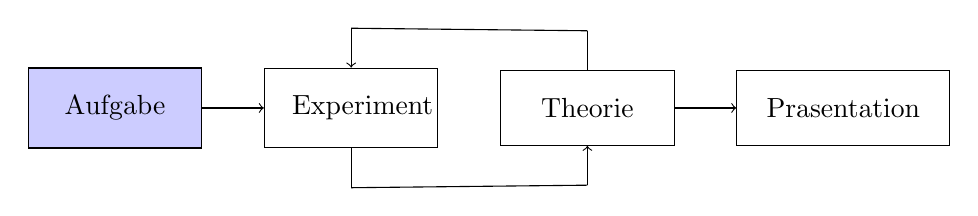
\begin{tikzpicture}

\node[draw, inner sep=10pt, text width=1.5cm, align=center, right, fill=blue!20!white] (2) at (-4, -2) {Aufgabe};
\node[draw, inner sep=10pt, text width=1.5cm, align=center, right, fill=white] (3) at (-1, -2) {Experiment};
\node[draw, inner sep=10pt, text width=1.5cm, align=center, right, fill=white] (4) at (2, -2) {Theorie};
\node[draw, inner sep=10pt, text width=2cm, align=center, right, fill=white] (5) at (5, -2) {Prasentation};

\draw[->] (2.east) -- (3.west);
\draw[->] (4.east) -- (5.west);

\draw (4.north) -- +(0, 0.5) coordinate (a);
\draw[<-] (3.north) -- +(0, 0.5) coordinate (b);
\draw (a) -- (b);

\draw[<-] (4.south) -- +(0, -0.5) coordinate (a);
\draw (3.south) -- +(0, -0.5) coordinate (b);
\draw (a) -- (b);

\end{tikzpicture}
\vfill
Problemstellungen sind offen formuliert
\begin{itemize}
\item alles was nicht ausgeschlossen ist, kann bearbeitet werden
\item[$\rightarrow$] kaum vollstaendig zu bearbeiten
\item[$\rightarrow$] koennen auf verschiedenen Schwierigkeitsstufen bearbeitet werden
\item[$\rightarrow$] \emph{realistischen} Fokus setzen!
\end{itemize}

Problem aussuchen ...
\begin{itemize}
\item abhaengig von Erfahrung und Praeferenz
\item ...zu empfehlen sind jedoch Mechanikprobleme (meine Meinung)
\end{itemize}
\end{frame}

\begin{frame}{Beispiel: \emph{Friction Oscillator}}

\textbf{Phaenomen}
{\large A massive \color{brown}object \color{black} is placed onto two identical parallel horizontal cylinders. The two cylinders each rotate with the same angular velocity, but in opposite directions.}
\vfill
\pause
\begin{center}
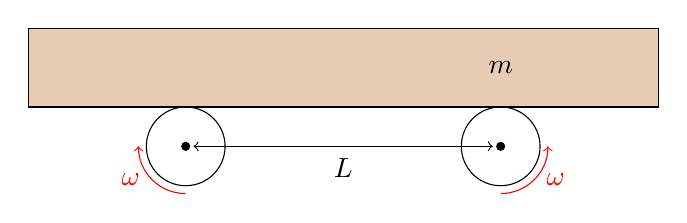
\begin{tikzpicture}
  \draw[fill=brown!40!white] (0, -0.5) -- (0, -1.5) -- (8, -1.5) -- (8, -0.5) -- (0, -0.5);
  \node at (6, -1) {$m$};
  \draw[<->] (2.1, -2) -- (5.9, -2) node[pos=0.5, below=1pt] {$L$};


  \draw (2, -2) circle [radius=0.5];
  \filldraw (2, -2) circle [radius=0.05];
  \draw (6, -2) circle [radius=0.5];
  \filldraw (6, -2) circle [radius=0.05];
  \draw[->, red] (6, -2)+(-90:0.6) arc [start angle=-90, end angle=0, radius=0.6] node[pos=0.5, right=1pt] {$\omega$};
  \draw[->, red] (2, -2)+(-90:0.6) arc [start angle=-90, end angle=-180, radius=0.6] node[pos=0.5, left=1pt] {$\omega$};
\end{tikzpicture}
\end{center}
\vfill
\pause
\textbf{Aufgabe}
{\large Investigate how the \color{blue}motion \color{black} of the object on the cylinders depends on the \color{orange}relevant \textbf{parameters}\color{black}.}
\end{frame}

\section{Experiment}

\begin{frame}{Erste Beobachtungen}
\includemedia[
  width=\textwidth,
  height=0.6\textwidth,
  activate=pageopen,
  addresource=videos/exp.mp4,
  flashvars={
   source=videos/exp.mp4
   &autoPlay=true
  }
]{}{VPlayer.swf}
\end{frame}


\begin{frame}{Experiment}
Experimenteller Aufbau sollte ...
\begin{itemize}
\item der Aufgabe entsprechen
\item auf eure Theorie anwendbar sein
\item \emph{relevante} Parameter unabhaengig varieren und messen koennen
\item reproduzierbar sein
\item eure Annahmen (Assumptions) bestaetigen
\item Fehlerquellen minimieren
\end{itemize}
\pause
\begin{itemize}
\item[$\rightarrow$] erfordert Kreativitaet und Geschick
\end{itemize}
\end{frame}


\begin{frame}{Experiment}
\begin{center}
\hspace*{-0.5cm}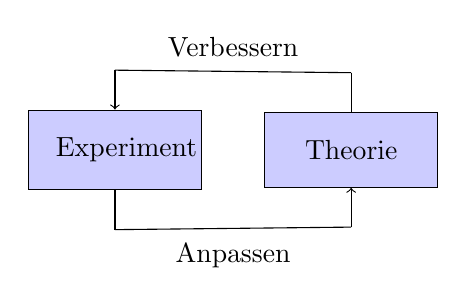
\begin{tikzpicture}

\node[draw, inner sep=10pt, text width=1.5cm, align=center, right, fill=blue!20!white] (3) at (-1, -2) {Experiment};
\node[draw, inner sep=10pt, text width=1.5cm, align=center, right, fill=blue!20!white] (4) at (2, -2) {Theorie};

\draw (4.north) -- +(0, 0.5) coordinate (a);
\draw[<-] (3.north) -- +(0, 0.5) coordinate (b);
\draw (a) -- (b) node[above=2pt, pos=0.5] {Verbessern};

\draw[<-] (4.south) -- +(0, -0.5) coordinate (a);
\draw (3.south) -- +(0, -0.5) coordinate (b);
\draw (a) -- (b) node[below=2pt, pos=0.5] {Anpassen};
\end{tikzpicture}
\end{center}

\vfill


Unter relevanten Parameter verstehen wir ...
\begin{itemize}
\item messbare Groeßen, die das Phaenomen beeinflussen
\item Ausgangsbedingungen (Initial conditions)
\item Randbedingungen (Boundray conditions)
\end{itemize}
 
\end{frame}

\begin{frame}{Beispiel: \emph{Friction Oscillator}}
  \resizebox{\textwidth}{!}{
  \begin{tikzpicture}
    \node[above right, inner sep=0] (image) at (0, 0) {
    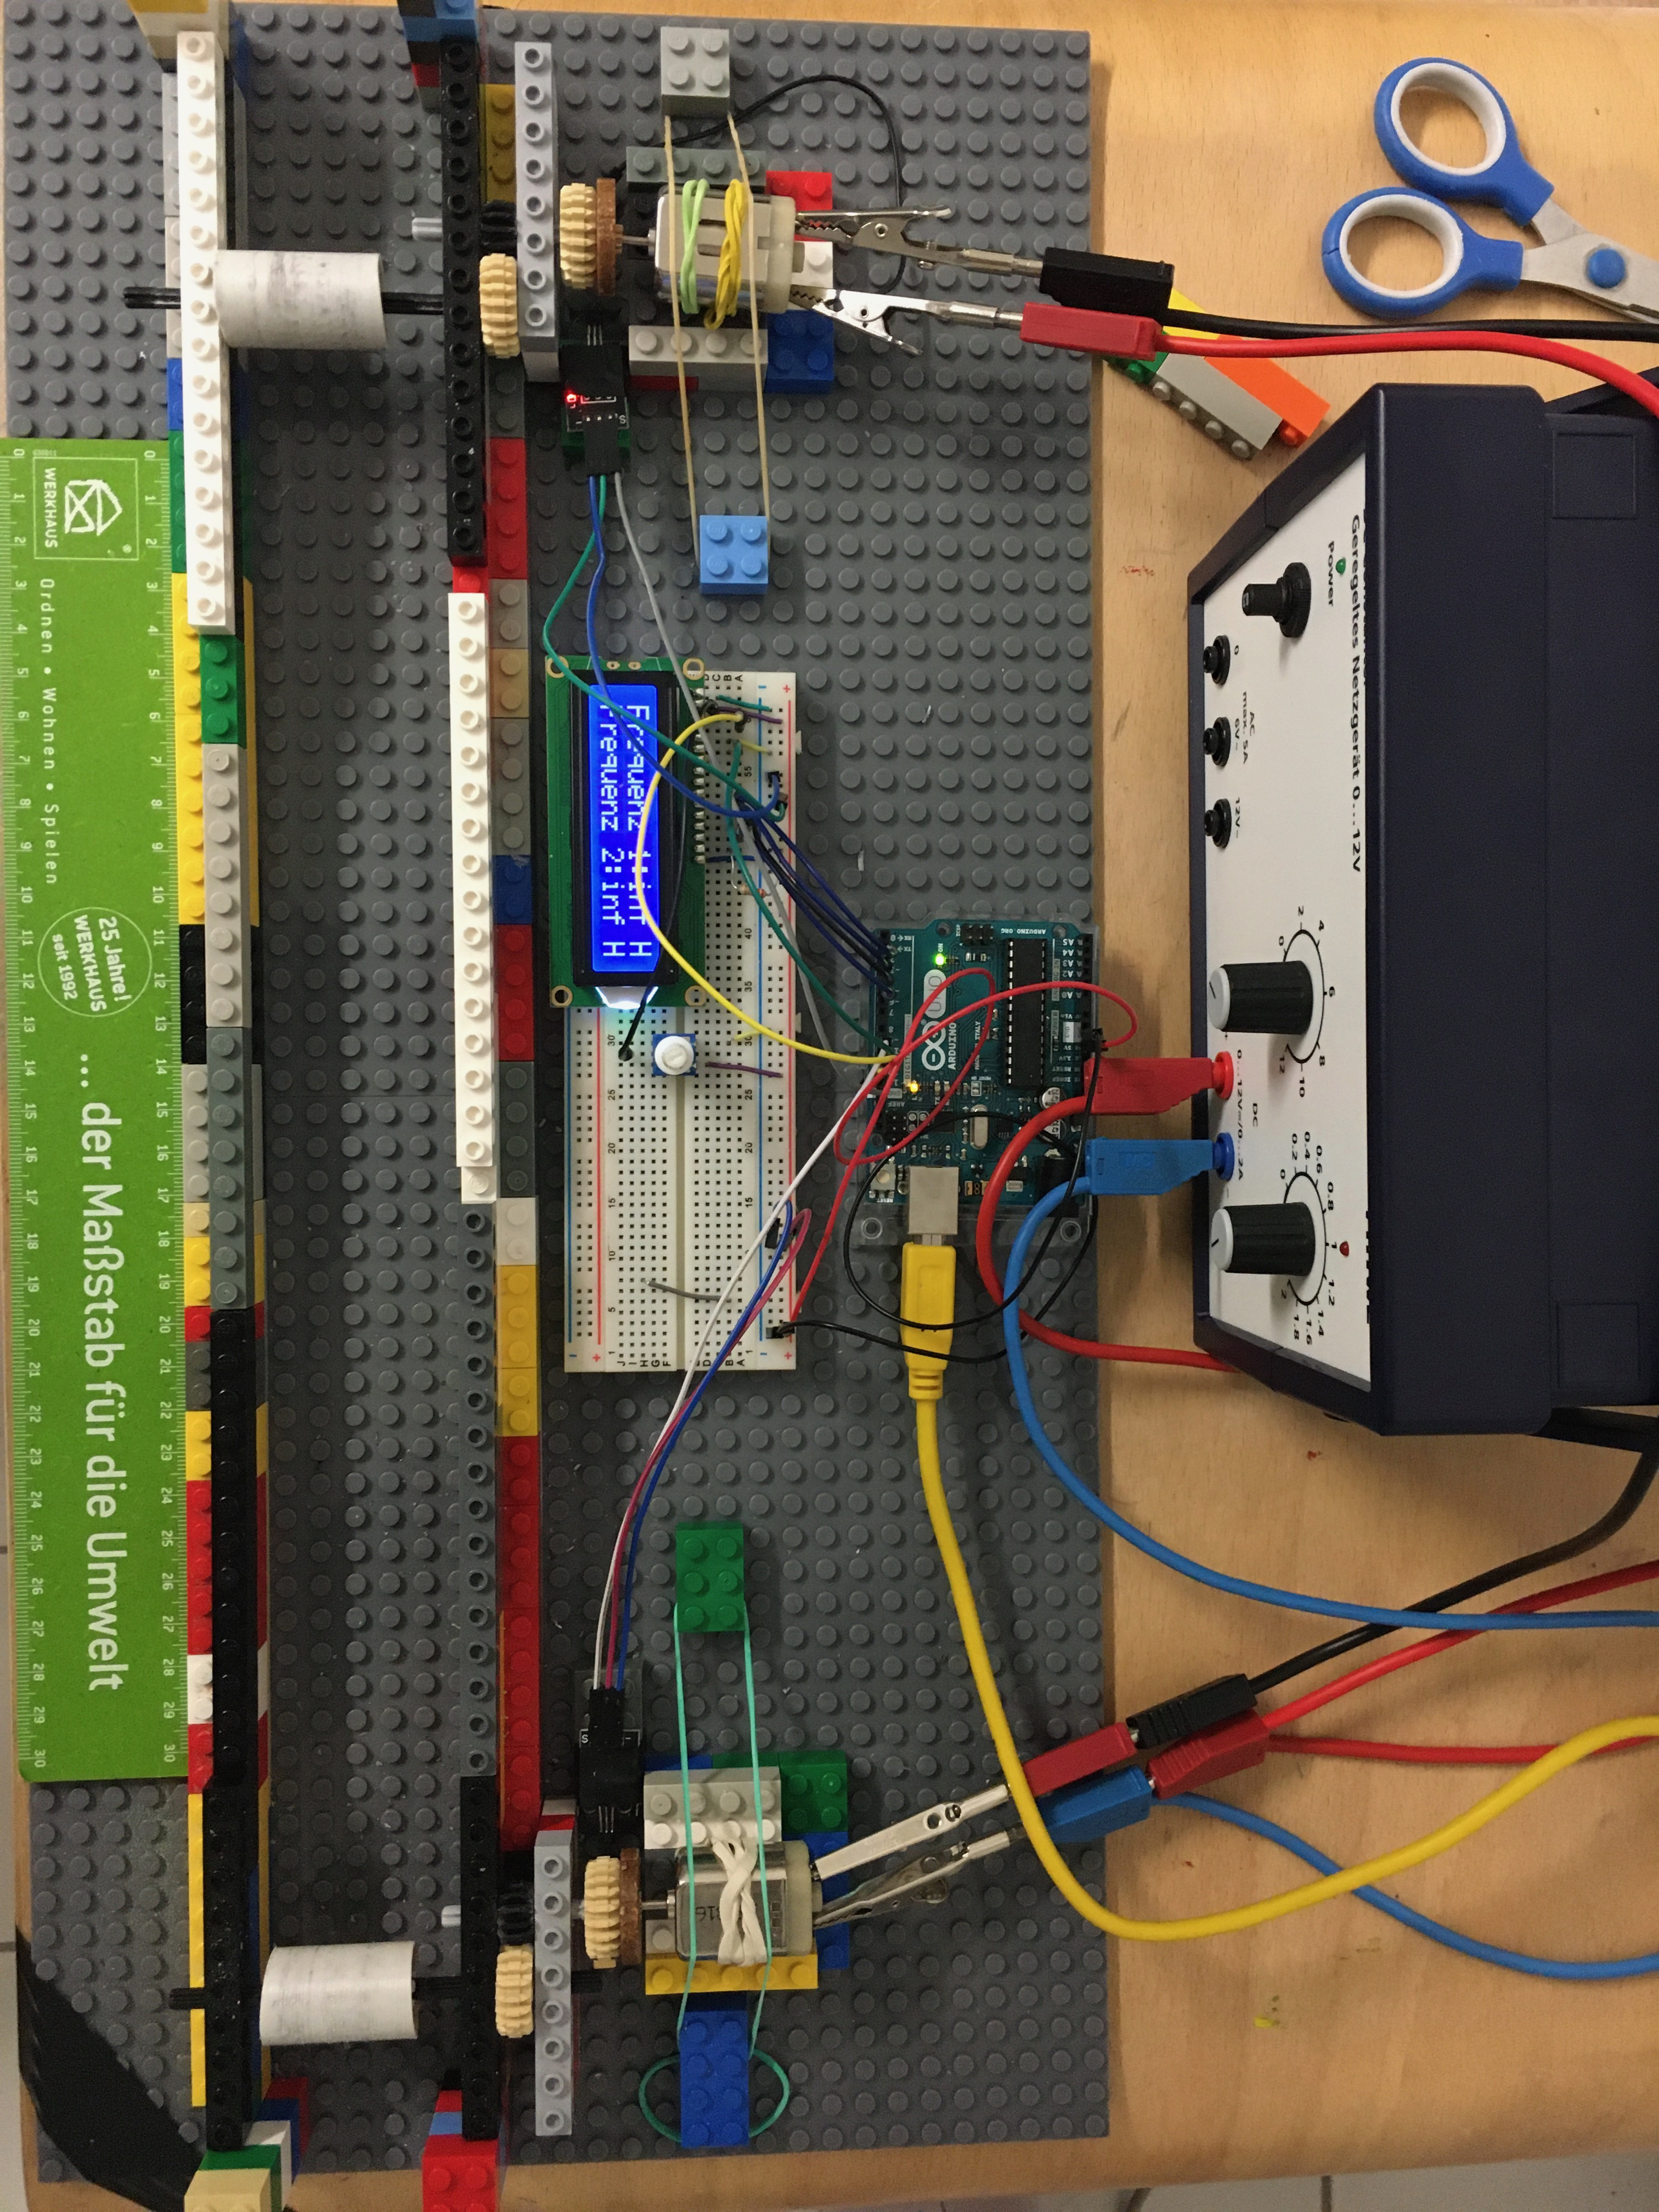
\includegraphics[width=\textwidth, angle=90]{photos/experiment}
    };
      \begin{scope}[
    x={($0.1*(image.south east)$)},
    y={($0.1*(image.north west)$)}]
     
    % Grid
    % \draw[lightgray,step=1] (image.south west) grid (image.north east);
     
    % Axes' labels
    % \foreach \x in {0,1,...,10} { \node [below] at (\x,0) {\x}; }
    % \foreach \y in {0,1,...,10} { \node [left] at (0,\y) {\y};}
     
    % Labels
        \node[black, fill=white] (cy) at (5, 2) {Zylinder};
        \node[black, fill=white] (el) at (5.5, 4.5) {Elektromotoren};
        \node[black, fill=white, below right] (hs) at (2, 3) {Hallsonde};
        \node[black, fill=white] at (4, 9) {Spannungsquelle};
        
        \node[below right,black,fill=white] at (4, 7) { Arduino};
        \draw[very thick, blue] (4, 5) rectangle (6, 7);
        \draw[very thick, blue, ->] (cy.west) -- (1.5, 2);
        \draw[very thick, blue, ->] (cy.east) -- (9, 2);
        \draw[very thick, blue, ->] (el.west) -- (1, 4.5);
        \draw[very thick, blue, ->] (el.east) -- (8.5, 4.5);
        \draw[very thick, blue, ->] (hs.north) -- (2, 3.5);
    \end{scope}
      
  \end{tikzpicture}
  }
\end{frame}

\begin{frame}{Parameter erkennen}
\textbf{Aufgabe}
{\large Investigate how the \color{blue}motion \color{black} of the object on the cylinders depends on the \color{orange}relevant \textbf{parameters}\color{black}.}
\vfill
\begin{center}
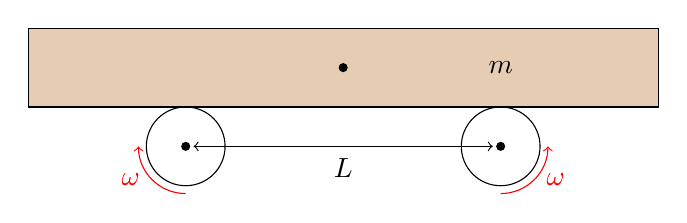
\begin{tikzpicture}
  \draw[fill=brown!40!white] (0, -0.5) -- (0, -1.5) -- (8, -1.5) -- (8, -0.5) -- (0, -0.5);
  \node at (6, -1) {$m$};
  \draw[<->] (2.1, -2) -- (5.9, -2) node[pos=0.5, below=1pt] {$L$};

  \filldraw (4, -1) circle[radius=0.05];
  \draw (2, -2) circle [radius=0.5];
  \filldraw (2, -2) circle [radius=0.05];
  \draw (6, -2) circle [radius=0.5];
  \filldraw (6, -2) circle [radius=0.05];
  \draw[->, red] (6, -2)+(-90:0.6) arc [start angle=-90, end angle=0, radius=0.6] node[pos=0.5, right=1pt] {$\omega$};
  \draw[->, red] (2, -2)+(-90:0.6) arc [start angle=-90, end angle=-180, radius=0.6] node[pos=0.5, left=1pt] {$\omega$};
\end{tikzpicture}
\end{center}
\vfill
\begin{columns}
\column{0.6\textwidth}
{\large \color{orange}\textbf{Parameter}\color{black}}
\column{0.4\textwidth}
{\large \color{blue}\textbf{Motion}\color{black}}
\end{columns}
\begin{columns}
\column{0.6\textwidth}
\begin{itemize}
\item Winkelgeschwindigkeit der Zylinder $\omega$
\item Zylinderabstand $L$
\item Masse $m$
\item Initiale Auslenkung $x_0$
\item Reibungskoeffizienten $\mu_s$ und $\mu_d$ 
\end{itemize}
\column{0.4\textwidth}
\begin{itemize}
\item Auslenkung $x$
\item Geschwindigkeit $\dot{x}$
\end{itemize}
\end{columns}
\end{frame}


\begin{frame}{Datenaufnahme und -auswertung}
  Zur Datenerhebung steht im Schuelerlabor ...
  \begin{itemize}
    \item Digitalkamera, Handy zur Video- und Audioaufnahme
    \item Waermebildkamera FLIR
    \item Kraftsensor, Multimeter, Thermometer, Hallsonde, ...
    \item Vernier DataQuest, GTR, ...
    \item ...
  \end{itemize}
  zur Verfuegung.
  \vfill
  \pause
  Datenanalyse haengt von Praeferenz, Erfahrung und Daten ab, 
  \begin{itemize}
    \item Tracker, OpenCV (Python, C++) fuer Videodaten
    \item FLIR Research IR
    \item Vernier DataLogger
    \item Audacity fuer Audiodaten
    \item Python Jupyter Lab, Excel, Mathematica zur Auswertung, etc.
  \end{itemize}
\end{frame}

\begin{frame}{Beispiel: \emph{Friction Oscillator}}
  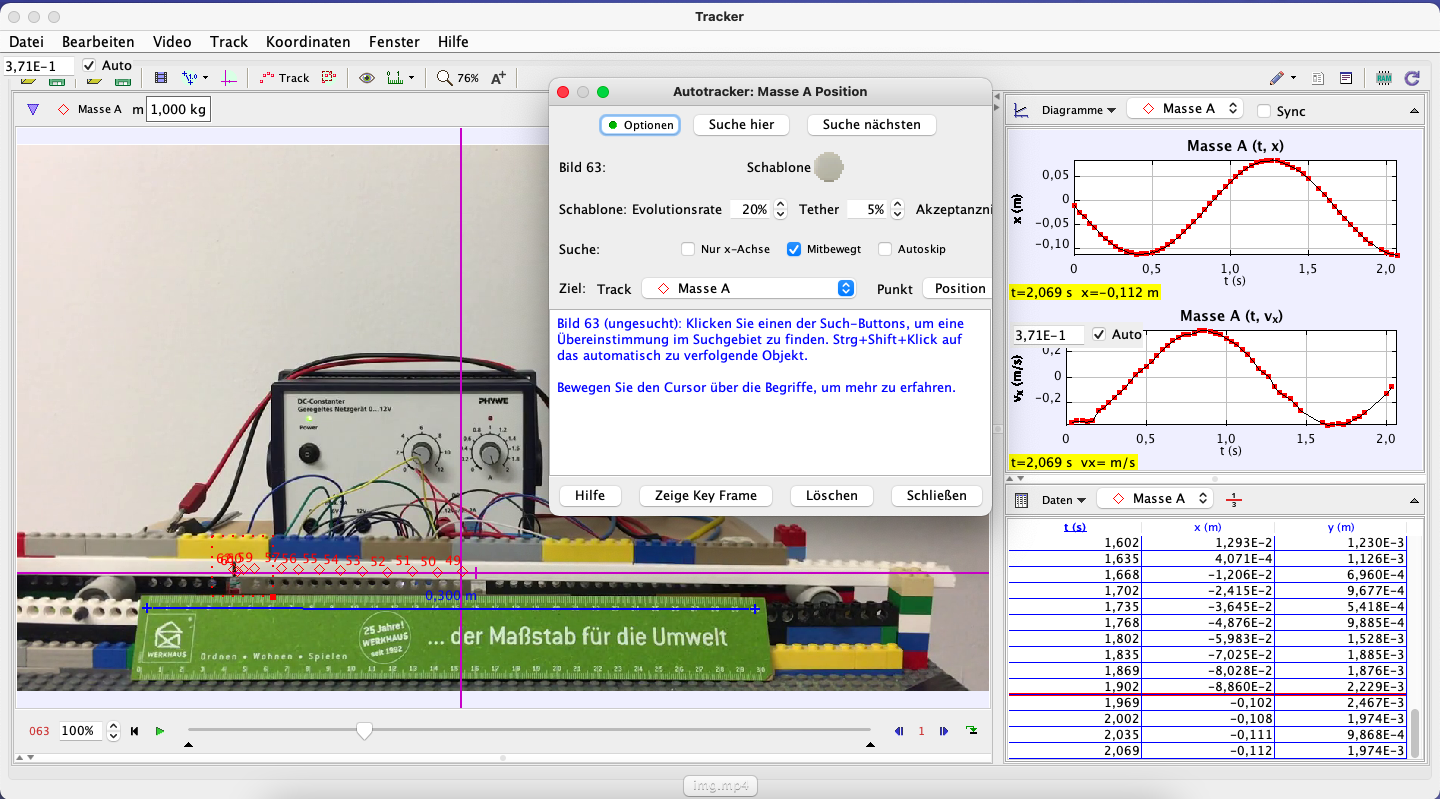
\includegraphics[width=\textwidth]{photos/screenshot}
  \begin{itemize}
    \item Position und Geschwindigkeit von Markierungen koennen mit Tracker ermittelt werden
    \item Daten werden dann exportiert
  \end{itemize}
\end{frame}

\begin{frame}{Beispiel: \emph{Friction Oscillator}}
  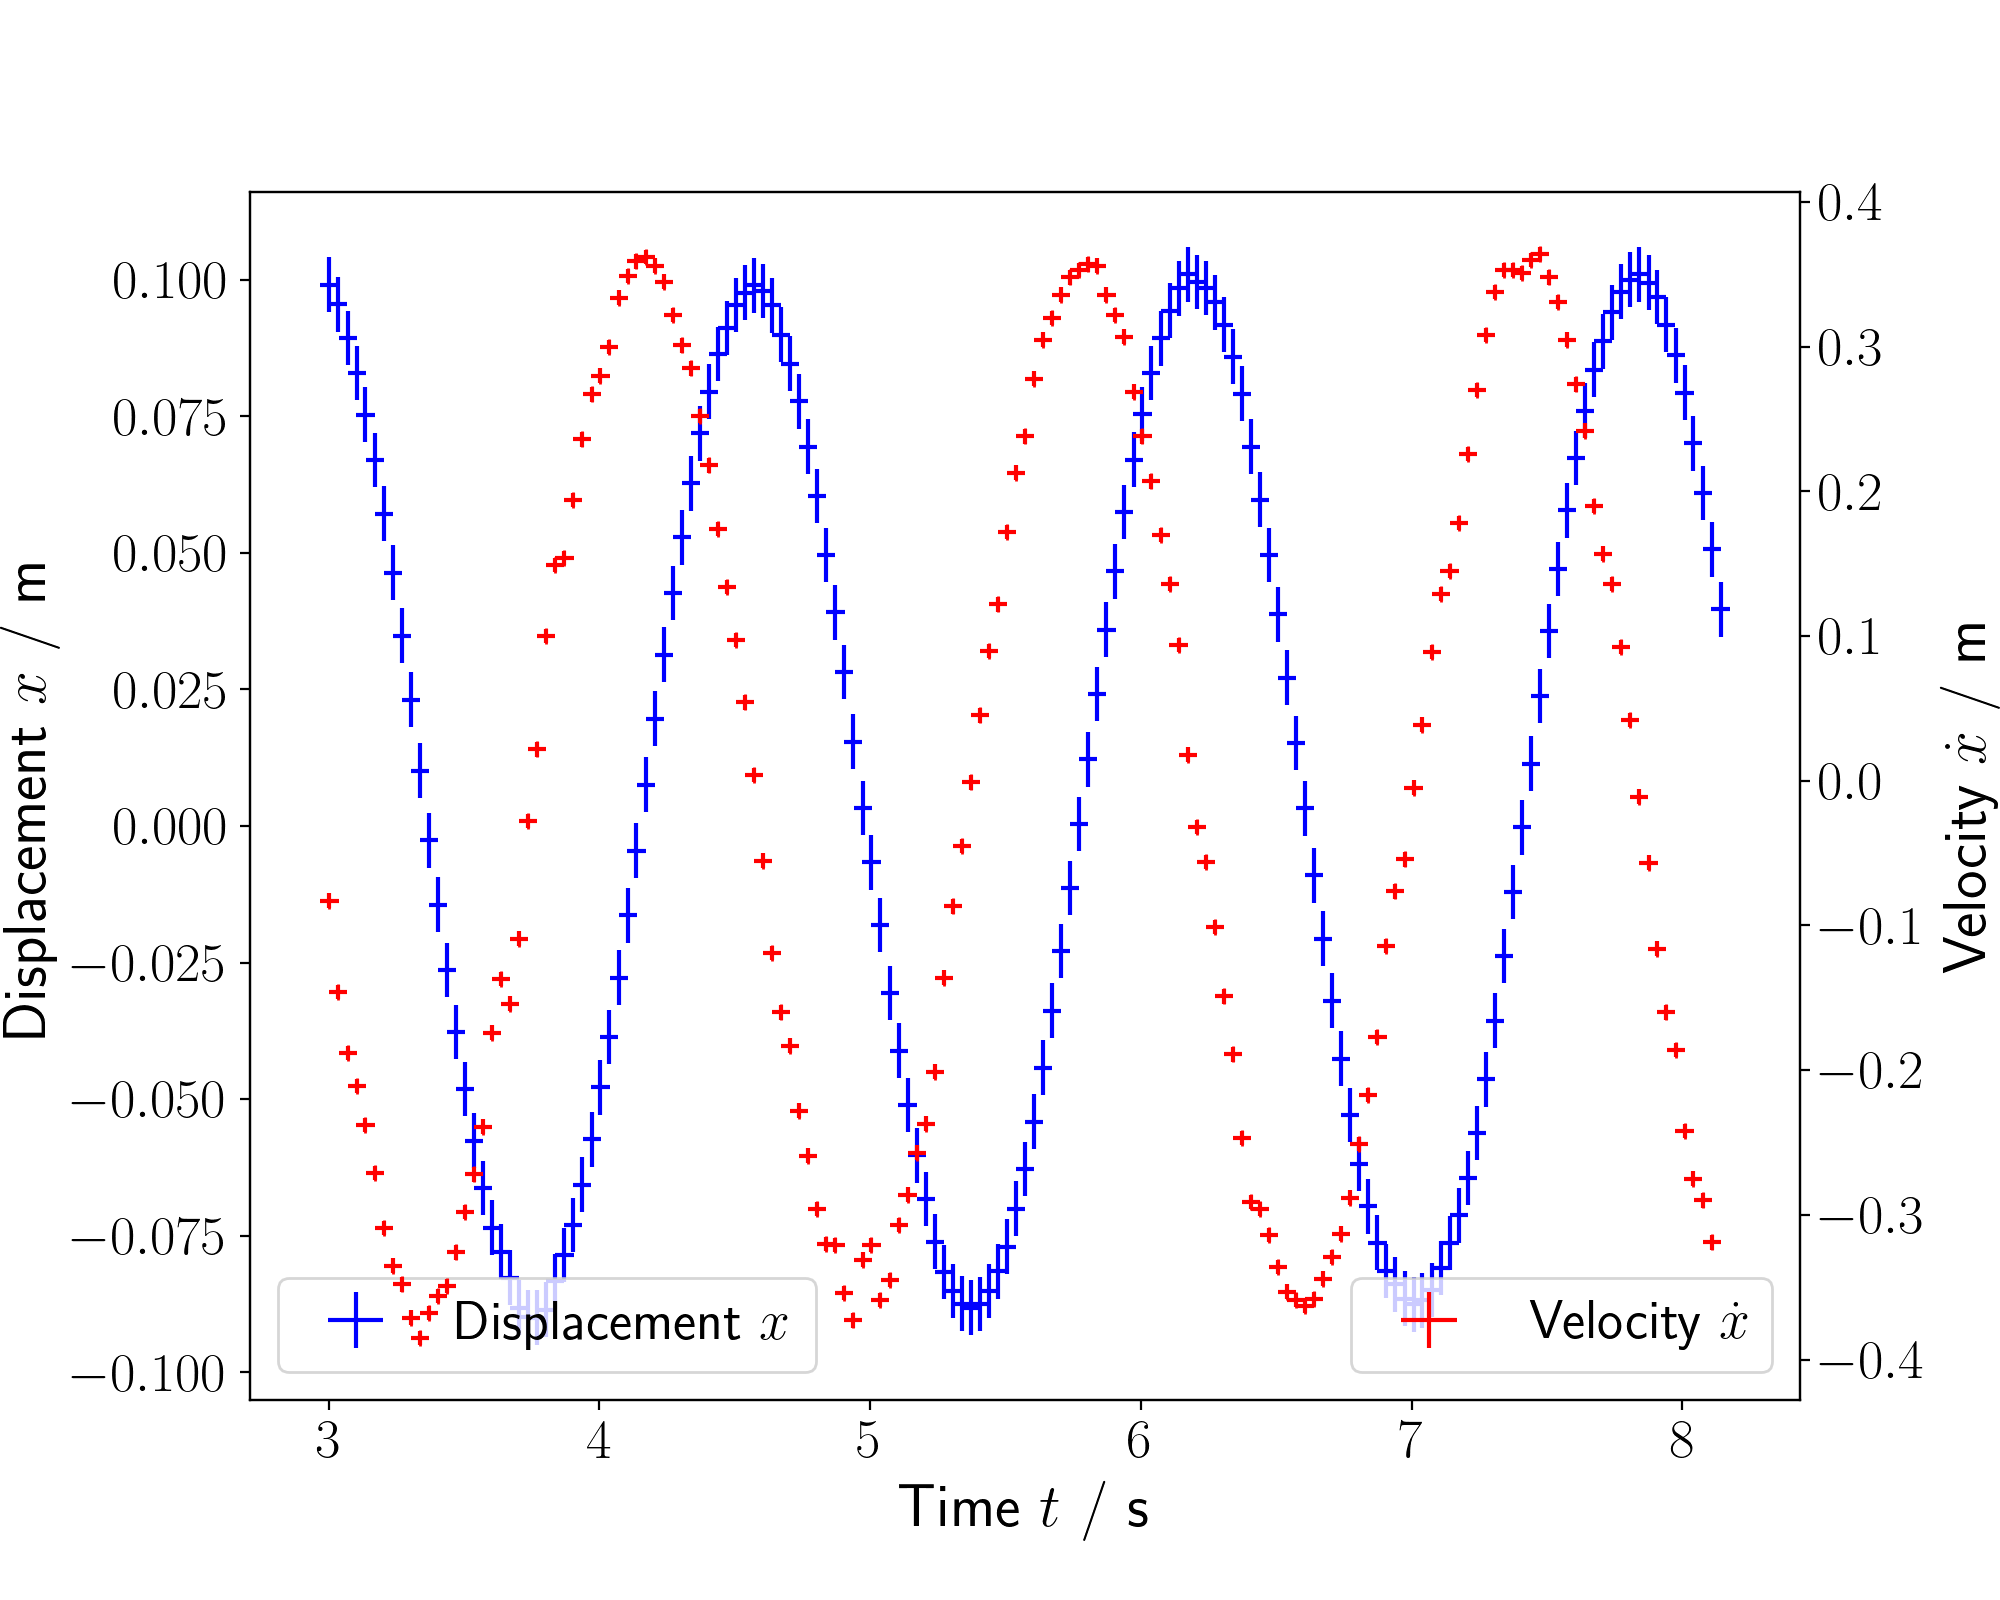
\includegraphics[width=\textwidth]{photos/oscillation}
  
\end{frame}

\section{Theorie}
\begin{frame}{Theorie: \emph{Qualitative Erklaerung}}
\begin{center}
{\large Die \textbf{Basic Explanation} erklaert in \underline{Worten} das Phaenomen.}
\end{center}
\pause\vfill

\begin{center}
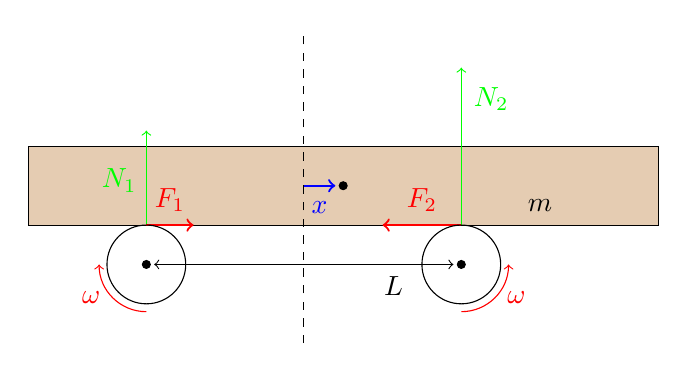
\begin{tikzpicture}
  \draw[fill=brown!40!white] (0.5, -0.5) -- (0.5, -1.5) -- (8.5, -1.5) -- (8.5, -0.5) -- (0.5, -0.5);
  \filldraw (4.5, -1) circle [radius=0.05];
  \node at (7, -1.25) {$m$};
  \draw[<->] (2.1, -2) -- (5.9, -2) node[pos=0.8, below=1pt] {$L$};
  \draw[green, ->] (2, -1.5) -- +(0, 1.2) node[pos=0.5, below=1pt, left] {$N_1$};
  \draw[thick, red, ->] (2, -1.5) -- +(0.6, 0) node[pos=0.5, above=1pt] {$F_1$};
  \draw[green, ->] (6, -1.5) -- +(0, 2) node[pos=0.8, right=1pt] {$N_2$};
  \draw[thick, red, ->] (6, -1.5) -- +(-1, 0) node[pos=0.5, above=1pt] {$F_2$};
  \draw[dashed] (4, -3) -- (4, 1);
  \draw[thick, blue, ->] (4, -1) -- (4.4, -1) node [blue, pos=0.5, below=2pt] {$x$};

  \draw (2, -2) circle [radius=0.5];
  \filldraw (2, -2) circle [radius=0.05];
  \draw (6, -2) circle [radius=0.5];
  \filldraw (6, -2) circle [radius=0.05];
  \draw[->, red] (6, -2)+(-90:0.6) arc [start angle=-90, end angle=0, radius=0.6] node[pos=0.5, right=1pt] {$\omega$};
  \draw[->, red] (2, -2)+(-90:0.6) arc [start angle=-90, end angle=-180, radius=0.6] node[pos=0.5, left=1pt] {$\omega$};
\end{tikzpicture}
\end{center}


\par
\textbf{Friction Oscillator}
\par
\begin{itemize}
\item Auslenkung fuehrt zu Kraefteungleichgewicht
\item[$\rightarrow$] Ruecktreibende Kraft wirkt beschleunigend
\item[$\rightarrow$] Traegheit des Objekts bewirkt erneute Auslenkung ueber Gleichgewichtslage
\end{itemize}
\end{frame}

\begin{frame}{Theorie: \emph{Quantitative Beschreibung}}
\begin{center}
{\large \textbf{Quantitative Analyse} beschreibt physikalische Phaenomene mathematisch.}
\end{center}

\vfill
Abhaengig von Erfahrung und Problem:
\begin{itemize}
\item Literatursuche (Google Scholar, ResearchGate, Nature etc.)
\item Annahmen benennen und experimentell untersuchen ( z.B. schlupffreies Rollen, laminarer Fluss etc.)
\item evtl. verbessern / vergleichen von Modellen aus der Literatur
\item je nach eigener Erfahrung: Aufstellen von eigenen Modellen

\end{itemize}
\end{frame}

\begin{frame}{Beispiel: \emph{Friction Oscillator}}
\textbf{Annahmen}:
\begin{itemize}
  \item kein Rollen $\rightarrow$ Gleitreibung ($\mu_d$)
  \item $\mu_d = $ const.
\end{itemize}
\begin{columns}
\column{0.6\textwidth}
\resizebox{\columnwidth}{!}{ 
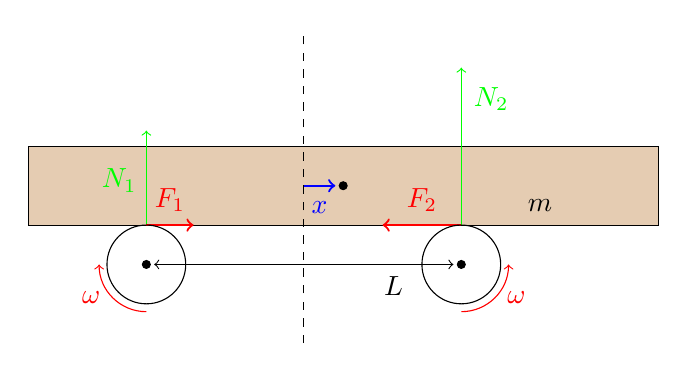
\begin{tikzpicture}
  \draw[fill=brown!40!white] (0.5, -0.5) -- (0.5, -1.5) -- (8.5, -1.5) -- (8.5, -0.5) -- (0.5, -0.5);
  \filldraw (4.5, -1) circle [radius=0.05];
  \node at (7, -1.25) {$m$};
  \draw[<->] (2.1, -2) -- (5.9, -2) node[pos=0.8, below=1pt] {$L$};
  \draw[green, ->] (2, -1.5) -- +(0, 1.2) node[pos=0.5, below=1pt, left] {$N_1$};
  \draw[thick, red, ->] (2, -1.5) -- +(0.6, 0) node[pos=0.5, above=1pt] {$F_1$};
  \draw[green, ->] (6, -1.5) -- +(0, 2) node[pos=0.8, right=1pt] {$N_2$};
  \draw[thick, red, ->] (6, -1.5) -- +(-1, 0) node[pos=0.5, above=1pt] {$F_2$};
  \draw[dashed] (4, -3) -- (4, 1);
  \draw[thick, blue, ->] (4, -1) -- (4.4, -1) node [blue, pos=0.5, below=2pt] {$x$};

  \draw (2, -2) circle [radius=0.5];
  \filldraw (2, -2) circle [radius=0.05];
  \draw (6, -2) circle [radius=0.5];
  \filldraw (6, -2) circle [radius=0.05];
  \draw[->, red] (6, -2)+(-90:0.6) arc [start angle=-90, end angle=0, radius=0.6] node[pos=0.5, right=1pt] {$\omega$};
  \draw[->, red] (2, -2)+(-90:0.6) arc [start angle=-90, end angle=-180, radius=0.6] node[pos=0.5, left=1pt] {$\omega$};
\end{tikzpicture}
}
\column{0.4\textwidth}
Nach Newtons zweitem Gesetz $F = m\ddot{x}$
\begin{equation*}
m \color{blue}\ddot{x}\color{black} = \color{red}F_1 \color{black} - \color{red}F_2 \color{black}
\end{equation*}
\end{columns}


\begin{columns}
\column{0.5\textwidth}
\begin{equation*}
F_1 = \mu_d N_1 = \mu_d \frac{\frac{L}{2} - x}{L} m g
\end{equation*}
\column{0.5\textwidth}
\begin{equation*}
F_2 = \mu_d N_2 = \mu_d \frac{\frac{L}{2} + x}{L} m g
\end{equation*}
\end{columns}

\begin{equation*}
\boxed{\ddot{x} = -\frac{2\mu_d g}{L} x}
\end{equation*}
\pause
\begin{itemize}
\item[$\rightarrow$] DGL eines harmonischen Oszillators ($\ddot{x} \propto x$) 
\item[$\rightarrow$] mit Eigenfrequenz $\omega_s = \sqrt{2 \mu_d \frac{g}{L}}$
\end{itemize}
\end{frame}


\begin{frame}{Theorie Experiment Vergleich}
\begin{center}
\hspace*{-0.5cm}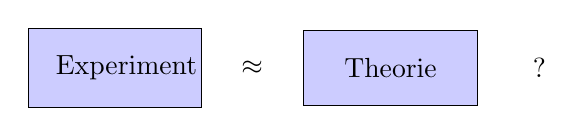
\begin{tikzpicture}

\node[draw, inner sep=10pt, text width=1.5cm, align=center, right, fill=blue!20!white] (3) at (-1, -2) {Experiment};

\node[align=center] at (1.85, -2) {$\approx$};

\node[draw, inner sep=10pt, text width=1.5cm, align=center, right, fill=blue!20!white] (4) at (2.5, -2) {Theorie};
\node[align=center] at (5.5, -2) {?};

\end{tikzpicture}
\end{center}
\vfill
Passt die Theorie zum Experiment ?
\begin{itemize}
\item[$\rightarrow$] je nach Problem der \underline{wichtigste} Schritt!
\item[$\rightarrow$] am besten durch Plots verdeutlichen (Excel, GNUPlot, Matplotlib, ...)
\item ... wenn nicht, koennen die Fehler erklaert werden ?
\item ... koennen Proportionalitaeten nachgewiesen werden ?
\end{itemize}
\end{frame}

\begin{frame}{Beispiel: \emph{Friction Oscillator}}
  \begin{center}
  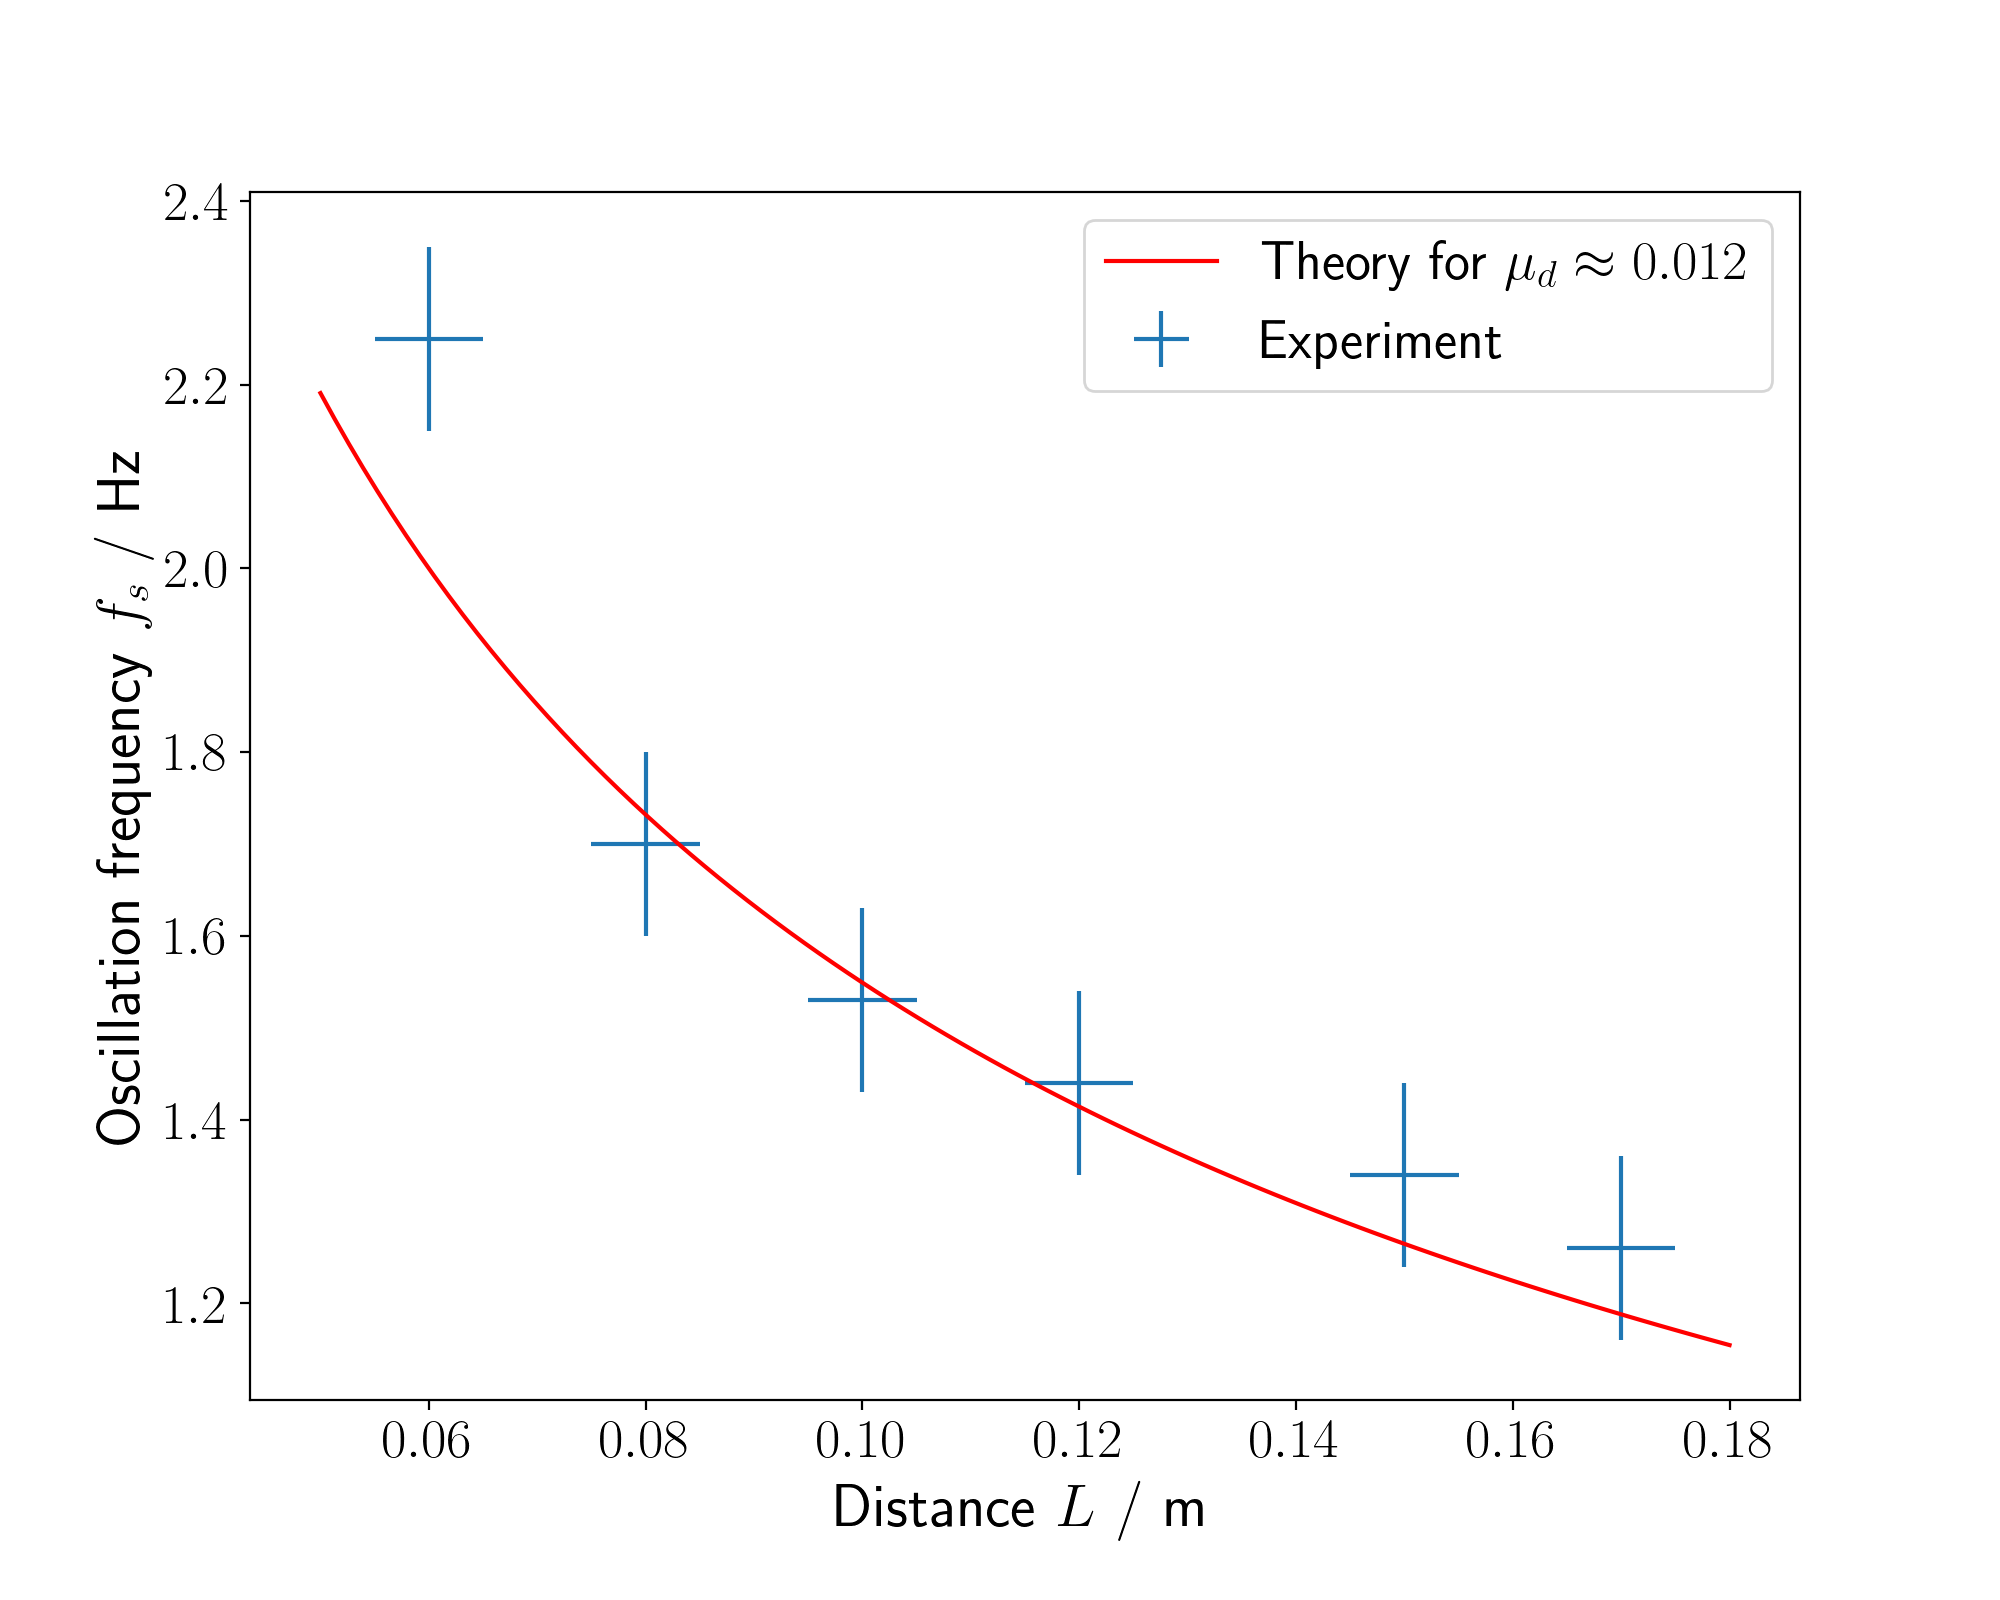
\includegraphics[width=0.8\textwidth]{photos/plot} 
  \end{center}
  \begin{itemize}
    \item Achsenbeschriftung (Formelzeichen, Einheiten, ...)
    \item Legende
    \item Datenpunkte mit Fehlerbalken (Standardabweichung, Messungenauigkeit, ...)
  \end{itemize}
\end{frame}

\begin{frame}{Anforderungen}
\end{frame}


\section{Diskusion}

\section{Juryfragen}

\begin{frame}{Timeline}
\begin{center}
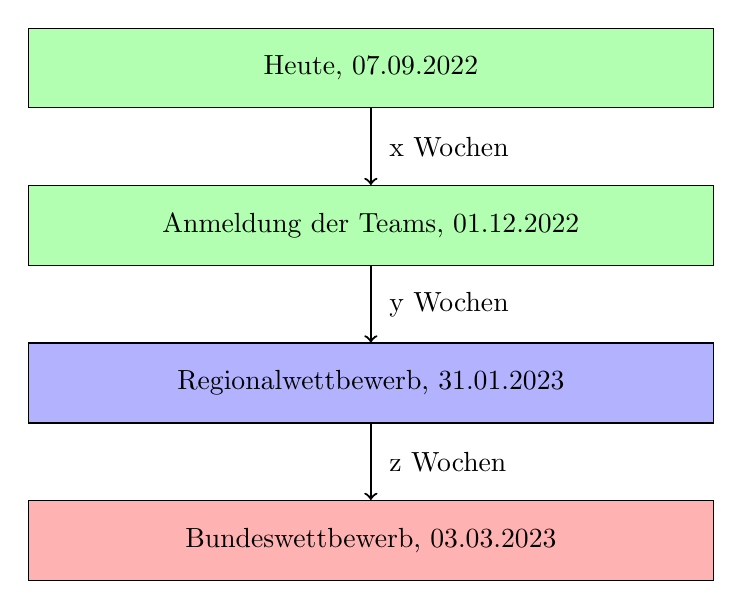
\begin{tikzpicture}
\node[align=center, inner sep=10pt, fill=green!30!white, draw, text width=8cm] (1) at (0, 0) {Heute, 07.09.2022};
\node[align=center, inner sep=10pt, fill=green!30!white, draw, text width=8cm] (2) at (0, -2) {Anmeldung der Teams, 01.12.2022};
\node[align=center, inner sep=10pt, fill=blue!30!white, draw, text width=8cm] (3) at (0, -4) {Regionalwettbewerb, 31.01.2023};
\node[align=center, inner sep=10pt, fill=red!30!white, draw, text width=8cm] (4) at (0, -6) {Bundeswettbewerb, 03.03.2023};


\draw[->, thick] (1.south) -- (2.north) node[pos=0.5, right=3pt] {x Wochen};
\draw[->, thick] (2.south) -- (3.north) node[pos=0.5, right=3pt] {y Wochen};
\draw[->, thick] (3.south) -- (4.north) node[pos=0.5, right=3pt] {z Wochen};

\end{tikzpicture}
\end{center}
\end{frame}

\end{document}
